\documentclass[]{article}
\usepackage{url}
\usepackage{cite}
\usepackage{listings}
\usepackage{xcolor} % for setting colors
\usepackage{lmodern}
\usepackage{graphicx}
\usepackage{textcomp}
\usepackage{hyperref}
\usepackage{enumerate}
\usepackage[numbers]{natbib}	

% set the default code style
\lstset{
	frame=tb, % draw a frame at the top and bottom of the code block
	tabsize=4, % tab space width
	showstringspaces=false, % don't mark spaces in strings
	numbers=left, % display line numbers on the left
	commentstyle=\color{green}, % comment color
	keywordstyle=\color{blue}, % keyword color
	stringstyle=\color{red} % string color
}

%opening
\title{VTX token retire mechanism v0.0.1}
\author{
		Sylvain Cormier\\
	\texttt{sylvain@volentixlabs.com}
}


\begin{document}

\maketitle

\begin{abstract}

The Volentix token, VTX was originally created on the main EOSIO chain.
Volentix Labs is offering ethereum users a way to purchase VTX using wrapped tokens. 

\end{abstract}

\section{Introduction }
Wrapped tokens are each backed by an equal amount of another asset. In this case, a pool of ETH VTX tokens is backed by a pool of VTX tokens on EOS to which a corresponding amount of original VTX token was sent.
The synchronisation of the initial EOS VTX with ETH VTX is ensured by: 
	\begin{enumerate}
	\item An oracle script executed by the nodes on the Volentix network, constantly feeding an EOS contract with the ETH VTX balance, account name, timestamp, block info etc...
	\item A smart contract on EOS validating this balance 
	\item The retiring of EOS VTX by this contract according to the new approved balance
\end{enumerate}


\section{System flow}
In the EOS contract, an initial unique record of the ETH VTX balance is kept as a reference. This record is updated anytime the EOS contract determines the ETH pool balance has changed.
For this, the EOS contract is continuously fed the VTX balance of the corresponding VTX pool on ethereum by registered vdexnode oracles. The EOS contract inserts these balances in a circular buffer, determining how many consecutive similar balances there are to the last incoming balance. If it was the case that the last 2/3 of the transactions were the same, The difference between the last recorded unique balance record and the new ethereum balance is calculated and the amount is sent to be retired on from the from the total VTX supply on the EOS chain. 
 
 
 
\begin{figure}
\centering
	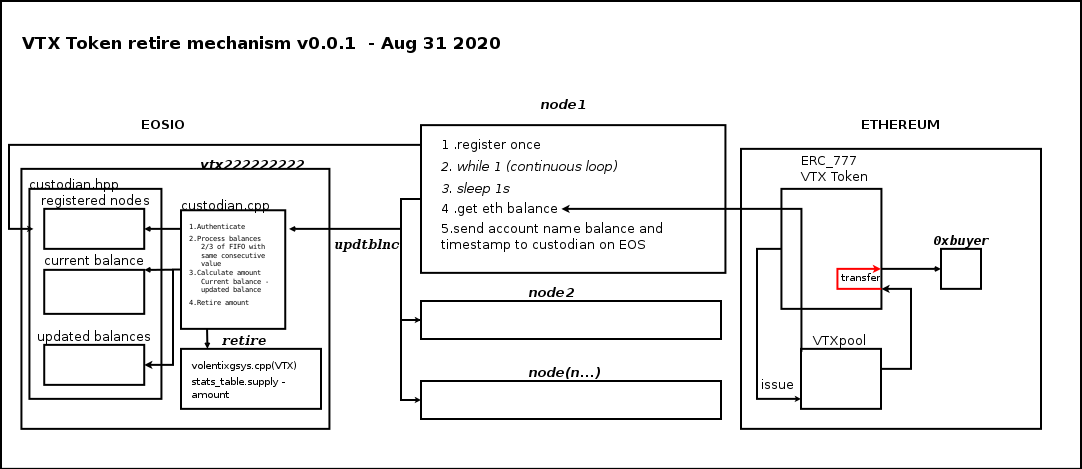
\includegraphics[scale=.33333]{bridge.png}
\caption{}
\label{fig:whitebackground-ecosystem02}
\end{figure}


\section{Conclusion}
Custodians trade assets for wrapped tokens by minting (creation of wrapped tokens) and burning (reducing supply of wrapped tokens). The latter has been accomplished in this iteration.
This mechanism can be used to to synchronize pools regardless of their provenances, as long as a the EOS contract is fed with the concerned balances.





\end{document}
